%%%%%%%%%%%%%%%%%%%%%%%%%%  ltexpprt.tex  %%%%%%%%%%%%%%%%%%%%%%%%%%%%%%%%
%
% This is ltexpprt.tex, an example file for use with the SIAM LaTeX2E
% Preprint Series macros. It is designed to provide double-column output. 
% Please take the time to read the following comments, as they document
% how to use these macros. This file can be composed and printed out for
% use as sample output.

% Any comments or questions regarding these macros should be directed to:
%
%                 Donna Witzleben
%                 SIAM
%                 3600 University City Science Center
%                 Philadelphia, PA 19104-2688
%                 USA
%                 Telephone: (215) 382-9800
%                 Fax: (215) 386-7999
%                 e-mail: witzleben@siam.org


% This file is to be used as an example for style only. It should not be read
% for content.

%%%%%%%%%%%%%%% PLEASE NOTE THE FOLLOWING STYLE RESTRICTIONS %%%%%%%%%%%%%%%

%%  1. There are no new tags.  Existing LaTeX tags have been formatted to match
%%     the Preprint series style.    
%%
%%  2. You must use \cite in the text to mark your reference citations and 
%%     \bibitem in the listing of references at the end of your chapter. See
%%     the examples in the following file. If you are using BibTeX, please
%%     supply the bst file with the manuscript file.
%% 
%%  3. This macro is set up for two levels of headings (\section and 
%%     \subsection). The macro will automatically number the headings for you.
%%
%%  5. No running heads are to be used for this volume.
%% 
%%  6. Theorems, Lemmas, Definitions, etc. are to be double numbered, 
%%     indicating the section and the occurence of that element
%%     within that section. (For example, the first theorem in the second
%%     section would be numbered 2.1. The macro will 
%%     automatically do the numbering for you.
%%
%%  7. Figures, equations, and tables must be single-numbered. 
%%     Use existing LaTeX tags for these elements.
%%     Numbering will be done automatically.
%%   
%%
%%%%%%%%%%%%%%%%%%%%%%%%%%%%%%%%%%%%%%%%%%%%%%%%%%%%%%%%%%%%%%%%%%%%%%%%%%%%%%%



\documentclass[twoside,leqno,twocolumn]{article}  
\usepackage{ltexpprt} 

\begin{document}


%\setcounter{chapter}{2} % If you are doing your chapter as chapter one,
%\setcounter{section}{3} % comment these two lines out.

\title{\Large Forecasting a Moving Target: Ensemble Models for ILI Case
  Count Predictions.\thanks{IARPA OSI.}}
\author{Neo\thanks{Wachoswki bros.} \\
\and 
Goku\thanks{Saiyaan}}
\date{}

\maketitle

 
%\pagenumbering{arabic}
%\setcounter{page}{1}%Leave this line commented out.

\begin{abstract}
  \small\baselineskip=9pt
  This is the text of my  abstract.
  Maximum number of words : 300.\\
  Maximum Keywords: 9.\\
\end{abstract}
 
\section{Introduction.}
% mainfile: ../ltexpprt.tex
Surveillance reports published by health organizations is one of the
main resources for monitoring Influenza like illness (ILI) cases and for
years have been used by healthcare officials for public reactions.
However, these surveillance reports are published with a considerable
delay and hence, it takes a long time for health threats to become
visible to health officials. Therefore, in recent years, various
approaches have been proposed in the literature for monitoring and
prediction of influenza epidemics based on data mining and network
dynamics methods. A considerable number of such methods are based on collecting
social signals by mining diverse data sources such as 
search engine query statistics \cite{ref1, ref2}, social
media ``chatter''~\cite{ref3, ref4, ref5, ref6, ref7} and news articles \cite{ref8},


%and weather data \cite{ref9, Shaman_orig_humidity_link, Shaman_humidity_USA}.
%A number of approaches use only one data
%source (such as \cite{ref1} and \cite{ref4}) while some solutions work
%based on multiple data sources (such as \cite{ref3} and \cite{ref10}). 

%Different solutions have been proposed for different purposes. In a
%number of solutions, the aim is to predict the actual number of ILI
%cases in a specific society \cite{ref2}, \cite{ref1}. These methods are mostly 
%based on classical regression algorithms. At the same time, some research
%~\cite{ref3, ref4} has been directed at monitoring the spatio-temporal distribution of ILI cases in
%a way that can be used by healthcare officials for public reaction
%. The dynamic behavior of epidemics in a
%population is also studied in a number of works in order to understand
%the way that disease propagates through people and between cities
%\cite{ref8}, \cite{ref11}.
One of the pioneering work in this new-found usage of non-tradional data sources 
was presented by Ginsberg et al.~\cite{ref2} when the predicted week ILI case counts
by tracking the volume of search engine queries. This work inspired a number of similar 
researches such ~\cite{ref1}, where Yuan et al. used search query data from Baidu (a popular
search engine in Chine) to detect influenza outbreaks. Both these works were based on finding 
correlation between search query volumes of different keywords with official ILI estimates 
of corresponding regions. Apart from using different data sources, 
these two work also differed on the actual regression model used. While the firsst one was based on 
logit-linear model, the second one uses a simple linear regression model. 

%In their approach, Ginsberg et al. build time
%series based on Google search queries to track weekly ILI counts. In
%addition to Google search trends, previously published values in CDC ILI
%reports are used to learn a simple regression model that predicts weekly
%influenza counts two weeks ahead of CDC ILI surveillance reports. 
%In their approach
%they use real-time search query results for specific keywords as well as
%official statistics of influenza to build a regression model that can
%predict influenza case count one or two weeks in advance. In addition to
%different data sources, this method differs from \cite{ref2} in terms of
%the used regression model. In \cite{ref2} a logit-linear model is used
%while \cite{ref1} uses a simple linear regression model.
Even real-time ILI detection~\cite{ref4} systems have been proposed by comparing 
real-time Twitter data with disease statistics to monitor and predict ILI and cancer 
in USA. This work also focusses on the importance of tracking both spatial and temporal 
data. A similar work was presented by Sugamaran and Voss~\cite{ref7} to analyze 
spatio-temporal spread of the West Nile Virus using Twitter Data. 
Historical news articles have also been used by Ewing et al. in
\cite{ref8} to study the spread of influenza pandemic. Authors used data
mining and network analysis methods for this purpose. Topics are modeled
by using latent Dirichlet allocation. In \cite{ref12}, Eggo et al. use a
gravity model for propagation of disease between cities. They used
Bayesian Markov Chain Monte Carlo methods to estimates parameters of
their model. %This method can be considered as a single data source
%solution that works with real-time Tweeter data. 

Apart from these ``social sources'', there has also been considerable work on 
correlating physical indicators such as climate data with influenza outbreaks. 
The primary advantage of such data sources is the fact that the effects are much 
more causal and less noisy. 
Shaman et. al. ~\cite{ref9, Shaman_orig_humidity_link, Shaman_humidity_USA} 
explored this area in detail and found absolute humidity to be a good indicator of 
influezna outbreaks.

While these works have helped in showcasing the importance of the varied 
``surrogate'' sources that can be used to predict and/or monitor ILI outbreaks, 
only a few works have aimed at combining mutiple data sources 
~\cite{ref10, ref3}.  These works are mainly dependent on social
media data as well as other publicly available data sources such as news 
articles, social media and clinical reports. However, to the best of our knowledge 
ours is the first work that aims at investigating both ``social indicators'' as well 
as ``physical indicators'' to predict the ILI incidence. While, the social indicators
can serve to elucidate more direct response from the society about prevalent ILI 
conditions, physical indicators such as humidity provide direct observance about 
the underlying ILI levels. 

Also, from our analysis we have found that the official estimates as reported by
agencies~\cite{PAHO:2013} are often lagged by several weeks and even when they
are reported, the reports are modified upto several weeks before the estimates 
are finalized. A real-time prediction system which is based on historical data
needs to handle this kind of variations in the offical estimates to get an 
accurate picture of the ILI conditions. Finally, most of the analysis have been 
retrospective and without a proper experimental validation framework.

In this paper we propose a novel matrix-factorization based regression method with 
nearest neighbor embedding to predict the ILI case counts. Our contributions can be listed
as:
\begin{itemize}
  \item We investigate both ``social indicators'' and ''physical indicators'' to 
    understand the efficacy of each kind of sources towards ILI prediction.
  \item We present a systematic way of investigating each individual source for possible 
    correlation with ILI by describing a novel matrix factorization based regression method
    using neighborhood embedding to account for 
    non-linear relations between the surrogates and the official ILI estimates.
  \item We investigate te efficacy of combining the these different sources at model 
    level vs. data level towards final accuracy.
  \item We propose different ways of handling uncertaininties in the official 
    estimates and factor these uncertainities in our prediction models.
  \item Finally, we present a detailed and prospective analysis of our proposed methods
    by comparing predictions from a near-hoirzon real time prediction system to 
    official estiamtes.
\end{itemize}

The rest of the paper is organized as follows: we touch upon some related works in 
Section~\ref{sec:related}, followed by a formal problem definition in Section~\ref{sec:problem},
and description of our regression framework in Section~\ref{sec:methods}. In Section~\ref{sec:ensemble}, 
we investigate the question of how best to combine multiple sources and present our strategies to 
handle the variance in official estimates in Section~\ref{sec:moving}. We conclude with detailed 
experiments in Section~\ref{sec:experiments}, correspoding results in Section~\ref{sec:results} and present
our conclusions in Section~\ref{sec:conclusions}.
 %In \cite{ref10}
%different data sources are compared based on different factors such as
%reliability and timeliness. Multiple data sources such as news articles,
%social media, and clinical reports are considered in this study. Authors
%also proposed an integrated framework for a health surveillance system
%that works with multiple data sources. 

%In \cite{ref3}, Denecke et al.
%proposed an event-based approach which can be used for early prediction
%of ILI threats \cite{ref3}. In their method (M-Eco) they consider
%multiple resources such as Tweeter, TV reports, online news articles,
%and blogs. M-Eco is a bi-lingual system that works with information in
%English and German and uses clustering to group documents in to
%clusters. These clusters are then interpreted as signals and used for
%event detection. The system is also based on supervised learning methods
%that rely on signal definitions which have been entered by user.


\section{Related Works.}
% mainfile: ../ltexpprt.tex
%In \cite{ref4}
%different types of analysis are used including spatial, temporal, and
%textual analysis. The purpose of spatial analysis is to determine the
%distribution of disease in US while temporal analysis is used for
%tracking the changes in number of tweets with specific keywords.
%Furthermore, text mining is used for tracking the popularity of disease
%types, symptoms, and treatments. Results of these analyses are
%visualized separately and can be used by healthcare officials. An almost
%similar approach was reported in \cite{ref7} that uses spatio-temporal
%analysis of Twitter data to monitor West Nile Virus. 

\begin{figure}[t] \centering
    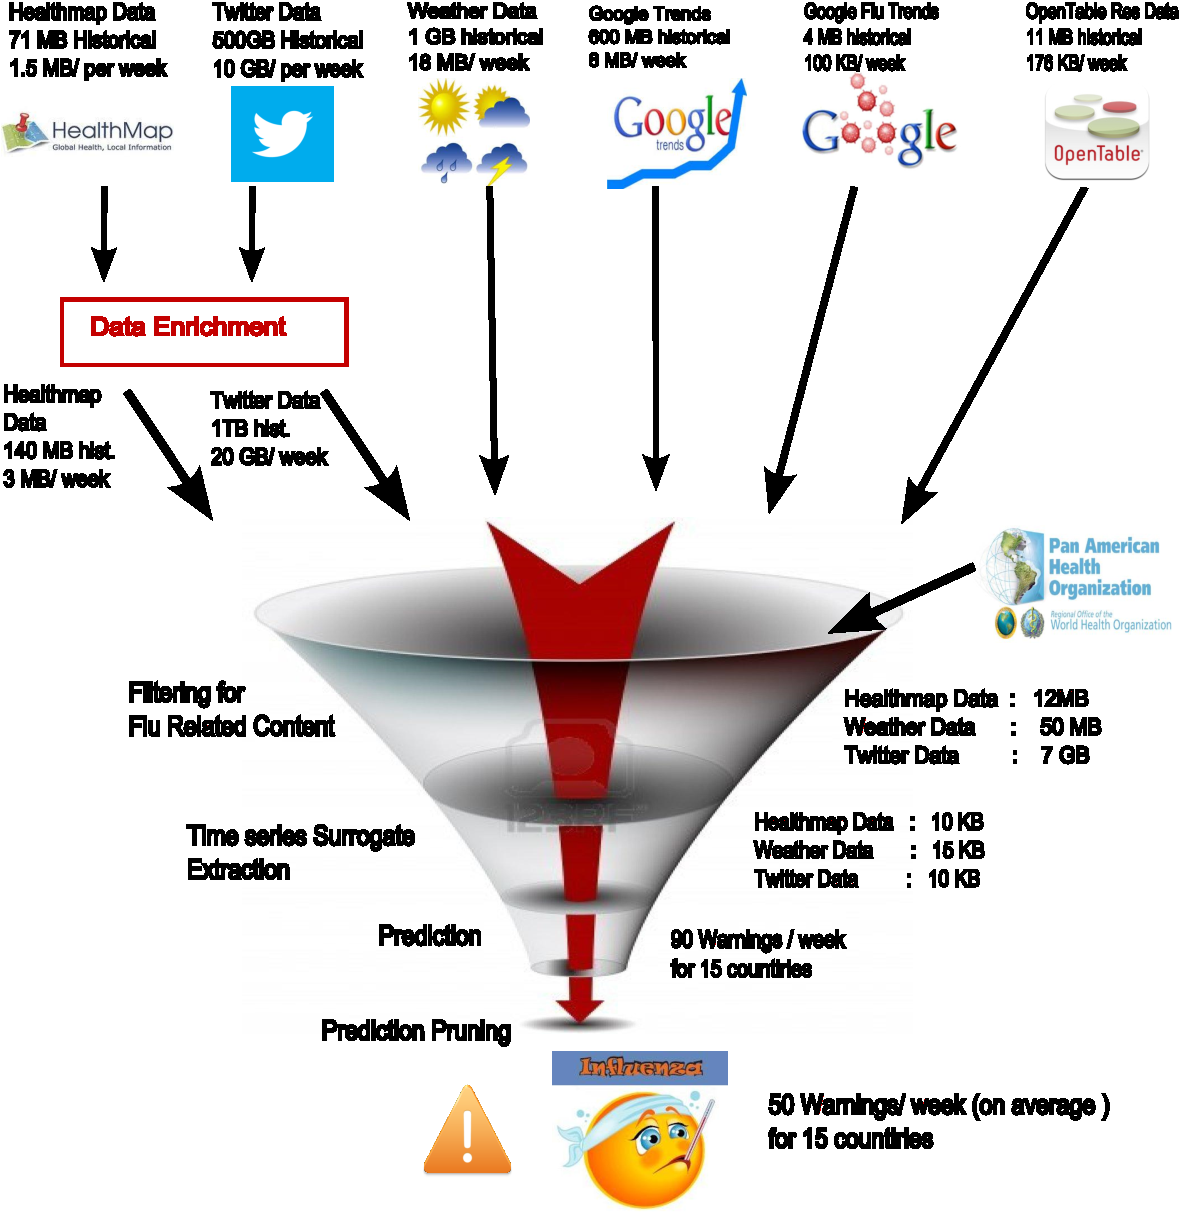
\includegraphics[scale=0.3]{fig/ili_data_pipeline.pdf}
    \caption{\label{fig:ili_data_pipeline} Our ILI data pipeline, depicting 
six different data sources used in this paper to forecast ILI case counts.}
 \end{figure}

Related work naturally falls into the categories of social media
analytics, physical indicators, and event dynamics modeling. 
 
\textbf{Social media analytics:}
Most work in social media analytics focuses on Twitter, specifically tracking
a dictionary of ILI-related keywords in the data stream.
Some investigations have focused on the importance of diversity in keyword 
lists, e.g.,~\cite{ref5, ref6}. In~\cite{ref5}, 
Kanhabua and Nejdl used clustering methods to determine
important topics in Twitter data, construct time series for matched keywords,
and used Jaccards coefficient to characterize the temporal
diversity of tweets. They note that such temporal diversity may be
correlated with real-world ILI outbreaks. In~\cite{ref6}
the authors study the dynamics of changes in tweets related to the H1N1 virus. We 
present our approach towards creating the keyword dictionary in Section~\ref{sec:keyword}.

\textbf{Physical indicators for detecting ILI incidence levels:} 
%One of the key indicators of ILI levels in a country is the prevalent 
%climactic patterns and the deviation from ``normal'' levels of these 
%indicators. For example 
Tamerius et al.~\cite{ref9} investigated the existence of seasonal 
cycles of influenza epidemics in different climate regions
by considering climatic information from 78 globally distributed sites. Through 
logistic regression they found out that, in cold-dry and humid-rainy
environments, strong correlation exists between influenza epidemics and
weather conditions. Similary exciting results were found 
by Shaman et. al.~\cite{Shaman_orig_humidity_link, Shaman_humidity_USA}
where they found absolute humidity to be a key indicator of flu. To uncover 
these relationships they used non-linear regressors such as Kalman filters.
and this was a key inspiration to us while finding an uniform model for the
vaired data sources as explained in Section~\ref{sec:methods}.

%\textbf{Non-linear regression methods:}
%There has been significant research in recommender systems to predict unknown user 
%ratings by combining techniques such as
%matrix factorization and nearest neighbor modeling. Although
%working essentially on categorical data, these methods are fine examples of non-linear
%regression methods which have been found to be robust as well as scalable (see~\cite{koren2008factor}).
%While matrix factorization have been long used (see ~\cite{canny2002factor}) to 
%connect the independent and dependent variables through latent factors, 
%recently Koren et al.~\cite{koren2008factor} presented detailed comparisons
%of nearest neighbors with matrix factorization methods and provided frameworks to 
%integrate the two approaches towards a unified non-linear predictor.
%
\textbf{Event dynamics modeling:}
Denecke et al.~\cite{ref3}
have proposed an event-based approach for early prediction
of ILI threats \cite{ref3}. In their method (M-Eco) they consider
multiple resources such as Twitter, TV reports, online news articles,
and blogs. M-Eco is a bi-lingual system that works with information in
English and German and uses clustering to identify signals for event detection.
Also, there exists related research in modeling the progression of influenza epidemics using
dynamical systems. Network dynamic solutions are used in~\cite{ref11} 
to study the behavior of an epidemic in a society. Spread of an infection through a network 
has been also studied as a general problem in graph mining, e.g., see~\cite{ref13,ref14}.
 


\section{Problem Specification.}
% mainfile: ../ltexpprt.tex

\iffalse
\begin{table*}[t!]
  \centering
  \begin{tabular}{|*{2}{l|}}
    \hline
    Abbreviation. & Description \\
    \hline \hline
    ${P}_t$         & Known ILI case count for time point $t$.\\
    $\hat{P}_t$     & Predicted ILI case count for time point $t$ \\
    $T$             & Max number of time points for which ILI case count is known.\\
    $\mathcal{X}_t$ & Surroagte data stream at time point $t$ .\\
    $T1$            & Max number of time points for which the surrogatedata streams are available.\\
    $\mathcal{F}_t$ & Google Flu Trends estimate at time point $t$ .\\
    $\mathcal{H}_t$ & Healthmap attributes at time point $t$ .\\
    $\mathcal{R}_t$ & Reservation data attributes at time point $t$ .\\
    $\mathcal{S}_t$ & Google Search Trends attributes at time point $t$.\\
    $\mathcal{T}_t$ & Twitter attributes at time point $t$ .\\
    $\mathcal{W}_t$ & Weather attributes at time point $t$ .\\
    $\alpha$        & Lookahead window length.\\
    $\beta$         & Lookback window length.\\
    $K$             & Maximum number of Nearest Neighbors.\\
    \hline
  \end{tabular}
  \caption{\label{tb:notations} Explanattions of notations used in the paper.
  \prithwish{May take this off later and put in the supplemental
section.}}
\end{table*}
\fi

Let
$\mathcal{P} = \langle {P}_1, {P}_2, \dots,{P}_T \rangle$
denote the known total weekly ILI case count for the country under
consideration, where ${P}_t$  denotes the case count for
time point $t$ and $T$ denotes the time point till which the
ILI case count is known.
%\prithwish{Will have to decide later whether we want to specify PAHO
  %here $\rightarrow$ \textnormal{``as reported by the Pan-American Health Organization
%(PAHO)~\cite{PAHO:2013}''}}\\
Corresponding to the ILI case count data, let us denote the available surrogate information
for the same country by 
$\mathcal{X} = \langle \mathcal{X}_1, \mathcal{X}_2, \dots, \mathcal{X}_{T1}\rangle$, 
where $T1$ is the time point till which the surrogate
information is available and $\mathcal{X}_{t}$ denotes the surrogate attributes for time
point $t$. 
The problem we desire to solve is to find a predictive model ($f$) for the 
case count data, as presented formally in Eqn~\ref{eq:problem}.
\begin{equation}
  \label{eq:problem}
  f: \mathcal{P}_t = f\left(\mathcal{P}, \mathcal{X}\right)
    \vspace{-2em}
\end{equation}



 
\section{Methods.}
% mainfile: ../ltexpprt.tex
%\prithwish{Resolve conflicts for \\
%1. ``time point'' vs ``time point''\\
%2. ``langle'' vs ``left(''}

We employ non-linear temporal regressions over the surrogate attributes to forecast the
case count using three broad models:
\begin{itemize}
  \item Matrix Factorizaiton Based Regression (MF).
  \item Nearest Neighbor Based Regression (NN).
  \item Matrix Factorization Regression using Nearest Neighbor embedding (MFN).
\end{itemize}
For each of the methods, we define two parameters: $\beta$ and $\alpha$. 
$\alpha$ is the {\it lookahead window length}, denoting distance of the time point for prediction from $T$;
$\beta$ is the {\it lookback window length} denoting the number of time points to look back
in order to find the regression relation between the case count and the surrogate data.

We define regression vectors $V_t$  and 
labels $L_t$ for all time points $t, \forall t = 1,\dots, T$
as given in equation~\ref{eq:regressionvector}.
%\prithwish{Check this}
\begin{equation}
  \label{eq:regressionvector}
  \begin{array}{lcl}
    V_t & \equiv & \langle P_{t-\beta - \alpha}, \mathcal{X}_{t-\beta - \alpha}, P_{t + 1 -\beta-\alpha}, \mathcal{X}_{t + 1 - \beta-\alpha}, \dots, \\
        &        & P_{t-\alpha},\mathcal{X}_{t-\alpha} \rangle \\
    L_t & \equiv & P_{t}\\
  \end{array}
\end{equation}
The regression vector for predicting the case count at time point $T' (T +
\alpha > T' > T)$ is given by equation~\ref{eq:regressiontestvector}.
\begin{equation}
  \label{eq:regressiontestvector}
  \begin{array}{lcl}
    V_{T'} & \equiv & \langle P_{T'-\beta - \alpha}, \mathcal{X}_{T'-\beta - \alpha}, P_{t + 1 -\beta-\alpha}, \mathcal{X}_{t + 1 - \beta-\alpha}, \dots, \\
           &        & P_{T'-\alpha},\mathcal{X}_{T'-\alpha} \rangle \\
  \end{array}
\end{equation}
\noindent
Under these definitions we describe the models as follows:
\subsubsection{\label{sec:model:matrixfactor} Matrix Factorization Based Regression (MF):}
Matrix Factorization is a well accepted technique in
the recommender systems literature, to predict user 
preferences from incomplete user ratings/informations. Typically~\cite{canny2002factor}
a user-preference matrix is factored into an user-factor and
factor-preference matrix. However, such factorizations are incognizant of any 
temporal continuity. As such to enforce temporal continuity, to predict for the time point 
$T' (T +\alpha > T' > T)$ we use the regression vectors 
and labels as defined in equation~\ref{eq:regressionvector} to define a $m \times n$ {\it prediction
matrix} $\mathcal{M}$, as given in equation~\ref{eq:predictionmatrix}:
\begin{equation}
  \label{eq:predictionmatrix}
\mathcal{M} = \left[\begin{array}{ll}
              V_{\alpha + \beta + 1} & L_{\alpha+\beta + 1} \\
                              \vdots & \vdots \\
                               V_{T} & L_T \\
                               V_{T'} & L_{T'} \\ 
    \end{array}
  \right]
\end{equation}

The prediction matrix is factorized into a $f\times m$ factor-feature matrix $U$ and 
a $f\times n$ factor-prediction matrix as:
\[ \widehat{\mathcal{M}}_{i,j} = b_{u,i} + U^T_i \times F_j\]
Here, $b_{i,j}$ is the baseline estimate given by:
 \begin{equation}
   \label{eq:baseline}
   b_{i,j} = \bar{\mathcal{M}} + b_j 
 \end{equation}
 where $\bar{\mathcal{M}}$ represents the all-element average and $b_j$ represents 
 the column wise deviations from the average and is generally a free-parameter, i.e.,
it is fitted as part of the optimization problem.
$U$ and $F$ matrix are estimated by minimizing the error function:
\begin{equation}
  \begin{array}{ll}
  \label{eq:matrix:fit}
  b_*, F, U  & =  \textrm{argmin} (\sum \limits_{i=1}^{m-1} \left(\mathcal{M}_{i,n}  - \widehat{\mathcal{M}}_{i,n} \right)^2 \\ 
  & + \lambda_1\times(\sum \limits_{j=1}^{n}b_j^2 + \sum \limits_{i=1}^{m-1} || U_i||^2 + \sum \limits_{j=1}^{n} || F_j||^2))
\end{array}
\end{equation}
\noindent
where $\lambda_1$ is a regularization parameter. An important design criteria in
the error function of Eqn~\ref{eq:matrix:fit} is the fact that we only compute the error
between the predicted label values and the actual label values i.e., the $n^{th}$ column of the prediction 
matrix $\mathcal{M}$. The rationale behind this choice is the fact that unlike traditional recommender 
systems we are only concerned with the label column and can sacrifice reconstruction accuracies for other 
columns. 

The lookback window $\beta$, the factor size $f$ and the regularization parameter $\lambda_1$ 
are estimated using cross-validation
and the final prediction for time point $T'$ is given by:
\[\widehat{P}_{T'} = b_{m,n} + U_m^T \times F_{m,n} \]

\subsubsection{\label{sec:model:nearestneighbor} Nearest Neighbor Based Regression (NN):}
For nearest neighbor models, we define a training set $\Gamma_{NN}
= \lbrace V_t, L_t \rbrace$, where $V_t$ represents the regression attributes
and $L_t$ denote the corresponding labels.
Also, let us define the set 
$\mathcal{N}(i) = \lbrace k : \mbox{$V_k$ is one of the top  K nearest neighbors of $V_{i}$} \rbrace$ 
where $K$ indicates the maximum number of nearest neighbors considered.
The predicted count $\widehat{P}_{T'}$ for the time point $T'$ is given as:
\begin{equation} \label{eq:nearestneighbor:pred}
  \begin{array}{lcl}
    \widehat{P}_{T'} & = & \frac{\sum\limits_{k \in \mathcal{N}(T')} \theta_{k}L_{k,T - \alpha}}
    {\sum\limits_{k=1}^{K} \theta_{k}}\\
  \end{array}
\end{equation}
%and $L_{k,T}$ indicates the label of the $k^{th}$ nearest neighbor to $V_{T'}$ in $\Gamma_{NN}$
%at time point $T$. 
\noindent
Here $\theta_k$ indicates the weight assigned to the $k^{th}$ nearest neighbor.
Typically the inverse Euclidean distances to $V_{T'}$ are chosen as the weights.

\subsubsection{\label{sec:model:nearestmatrix} Matrix Factorization Based
Regression using Nearest Neighbor Embedding (MFN):}
It has been shown in~\cite{koren2008factor} that matrix factorization using nearest neighbor constraints can
outperform classical matrix factorization approach as well as traditional nearest neighbor approaches towards
recommender systems. Here, we modify the method to suit the temporal nature of our problem in similar ways 
as described in section~\ref{sec:model:matrixfactor}. We again define a similar prediction matrix $\mathcal{M}$ 
(see equation~\ref{eq:predictionmatrix}). Following ~\cite{koren2008factor}, we define the 
matrix decomposition rule as 

\begin{equation}
  \label{eq:model:matrixfactornbr}
  \begin{array}{lcl}
    \widehat{\mathcal{M}}_{i,j} & = &  b_{i,j} + U_i^T\times F_j \\
                                &   & + F_j \times |\mathcal{N}(i)|^{-\frac{1}{2}}\sum_{k \in N(i)} (\mathcal{M}_{i,k} - b_{i,k}) x_k \\
  \end{array}
\end{equation}
\noindent
The key difference between equation~\ref{eq:model:matrixfactornbr} and the one proposed in 
~\cite{koren2008factor} is that we don't have any term for implicit feedback and, further,
only the top $K$ neighbors as found through Euclidean distance are used. 
The model is fitted using Eqn~\ref{eq:matrixnbr:fit} as given below:

\begin{equation}
  \label{eq:matrixnbr:fit}
  \begin{array}{ll}
    b_*, F, U, x_*  = \textrm{argmin} &(\sum \limits_{i=1}^{m-1} \left(\mathcal{M}_{i,n} - \widehat{\mathcal{M}}_{i,n}   \right)^2 \\
                    & + \lambda_2\times(\sum \limits_{j=1}^{n}b_j^2 + \sum \limits_{i=1}^{m-1} || U_i||^2 \\
                    & + \sum \limits_{j=1}^{n} || F_j||^2 + \sum_k ||x_k||^2))
  \end{array}
  \end{equation}



\section{Ensemble Approaches.}
% mainfile: ../ltexpprt.tex


Preliminary experiments shown that performance of neighborhood models for prediction of PAHO count values are better than other prediction methods. Hence, in this section, we propose an ensemble model based on nearest neighborhood regression models. For simplicity, we use subscripts $i$ and $j$ for indicating time slots (weeks). Known PAHO count values for week $i$ are shown by $P_{i}$ and predicted values are shown by $\hat{P}_{i}$. We assume that $\mathcal{P}$ is the set of all known PAHO count values for a specific country.

The first part of the model is to predict PAHO count values based on a simple averaging method. We name this basic averaging as baseline prediction. Then, baseline prediction is shown by $b$ and is determined as follows:

\begin{equation}
b = {1 \over {|\mathcal{P}|}} \sum_{i=1}^{|\mathcal{P}|}P_{i}
\end{equation}

where $|\mathcal{P}|$ is size of $\mathcal{P}$. 

Let us assume that we know the baseline prediction of a country and we want to predict PAHO count value for a specific week, $j$. Furthermore, assume that we want to use a generic data source, $\mathbb{D}$, for our predictions where $\vec{d}_i$ is a sample of $\mathbb{D}$ for week $i$. Each $\vec{d}_i$ is a vector of features and we show each element of $\vec{d}_i$ by $d_{ik}$. For the lookback window length $\beta$, to estimate the value of PAHO count for week $j$, PAHO counts of the last $\beta$ weeks ending at $j$ are used. Hence, PAHO count value for week $j$ is estimated as a function of $\vec{d}_{j-\beta+1}$, ..., $\vec{d}_{j}$, as follows:

\begin{equation}
\hat{P}_{j} = \mathit{f}(\vec{d}_{j-\beta+1},...,\vec{d}_{j})
\end{equation}

Distance between weeks $i$ and $j$ is determined as follows:

\begin{equation}
\Delta_{ij}^\mathbb{D} = \sqrt{\sum_{l=0}^{\beta-1} \sum_{k} (d_{k(i-l)}-d_{k(j-l)})^2}
\end{equation}

where $\Delta_{ij}^\mathbb{D}$ is the distance between weeks $i$ and $j$ based on generic dataset $\mathbb{D}$.

Let us assume that we have $n$ known PAHO values. In order to adjust the baseline prediction of week $j$, we measure $\Delta_{ij}^\mathbb{D}$ for all $n$ known weeks. $\mathcal{L}_{j}^\mathbb{D}$ is an ordered list, containing $n$ members, where the $i$th member is the $i$th nearest neighbor of week $j$. Then, we have:

\begin{equation}
\hat{P}_{j} = b + \sum_{i \in \mathcal{L}_{j}^\mathbb{D}}{} (P_i - b)w_{i}^\mathbb{D}
\label{eq:onesource}
\end{equation}

where, $w_{i}^\mathbb{D}$ is a constant weight for the $i$th nearest neighbor of week $j$. To determine these weights, one can solve the following optimization problem:

\begin{equation}
\min_{w_{*}^\mathbb{D}} \sum_{j \in \mathcal{P}} {(P_j - b - \sum_{i \in \mathcal{L}_{j}^\mathbb{D}}{} (P_i - b)w_{i}^\mathbb{D})^2} + \lambda \sum_{}{}{{(w_{i}^\mathbb{D})}^2}
\end{equation}

where, $\lambda \sum_{}{}{{(w_{i}^\mathbb{D})}^2}$ is the regularization term which is used to avoid over-fitting. This problem can be solved through a stochastic gradient descent algorithm.

If we have more than one dataset, one can use an ensemble method to combine the results of different predictors. Let us assume that we have two generic datasets, $\mathbb{D}1$ and $\mathbb{D}2$. Then, similar to Eq. ~\ref{eq:onesource}, we can use one dataset, $\mathbb{D}1$, to adjust the baseline prediction, and the other dataset to adjust the later prediction. This approach is illustrated in Eq. ~\ref{eq:twosource}:

\begin{equation}
\hat{P}_{j} = b + \sum_{i \in \mathcal{L}_{j}^{\mathbb{D}1}}{} (P_i - b)w_{i}^{\mathbb{D}1} + \sum_{i \in \mathcal{L}_{j}^{\mathbb{D}2}}{} (P_i - b - \sum_{k \in \mathcal{L}_{j}^{\mathbb{D}1}}{} (P_k - b)w_{k}^{\mathbb{D}1})w_{i}^{\mathbb{D}2}
\label{eq:twosource}
\end{equation}

where, $w_{i}^{\mathbb{D}1}$ and $w_{i}^{\mathbb{D}2}$ are constant weights for the $i$th nearest neighbors of week $j$ with respect to datasets $\mathbb{D}1$ and $\mathbb{D}2$. The following optimization problem can be solved to estimate these weights:

\begin{equation}
\min_{w_{*}^{\mathbb{D}1},w_{*}^{\mathbb{D}2}} \sum_{j \in \mathcal{P}} {(P_j - \hat{P}_j)^2} + \lambda (\sum_{}{}{{(w_{i}^{\mathbb{D}1})}^2}+\sum_{}{}{{(w_{i}^{\mathbb{D}2})}^2})
\label{eq:opt2}
\end{equation}


%\begin{equation}
%\min_{w_{*}^{\mathbb{D}1},w_{*}^{\mathbb{D}2}} \sum_{j \in \mathcal{P}} {(P_j - b - \sum_{i \in \mathcal{L}_{j}^{\mathbb{D}1}}{} (P_i - b)w_{i}^{\mathbb{D}1} - \sum_{i \in \mathcal{L}_{j}^{\mathbb{D}2}}{} (P_i - b - \sum_{k \in \mathcal{L}_{j}^{\mathbb{D}1}}{} (P_k - b)w_{k}^{\mathbb{D}1})w_{i}^{\mathbb{D}2})^2} + \lambda (\sum_{}{}{{(w_{i}^{\mathbb{D}1})}^2}+\sum_{}{}{{(w_{i}^{\mathbb{D}2})}^2})
%\label{eq:opt2}
%\end{equation}


where, $\hat{P}_j$ is determined based on Eq. ~\ref{eq:twosource}. In order to solve optimization problem of Eq. ~\ref{eq:opt2}, one can use stochastic gradient decent method. For this purpose, let us assume that $e_j$ is the error of prediction for week $j$, i.e. $e_j = P_j - \hat{P}_j$. Then, by going through the known values of PAHO count, we can update weights in the opposite direction of the gradient of Eq. ~\ref{eq:opt2} and we will have:

\begin{equation}
w_{i}^{\mathbb{D}1} \leftarrow w_{i}^{\mathbb{D}1}+ \gamma \left [e_j(P_i - b - (P_i - b) \sum_{k}{}{w_{i}^{\mathbb{D}2}}) + \lambda w_{i}^{\mathbb{D}1}  \right ]
\end{equation}
\begin{equation}
w_{i}^{\mathbb{D}2} \leftarrow w_{i}^{\mathbb{D}2}+ \gamma \left [e_j(P_i - b - \sum_{k}{}{(P_k - b)w_{k}^{\mathbb{D}1}}) + \lambda w_{i}^{\mathbb{D}2}  \right ]
\end{equation}

where $\gamma$ is a constant variable that determines step size of optimization. Parameters $\gamma$ and $\lambda$ are determined through cross validation.

For more than two datasets, a similar combining method can be used. It should be noted that order of datasets in Eq. ~\ref{eq:twosource} (and ensembles based on more datasets) is important and can be determined through cross validation.


\section{Forecasting a Moving Target.}
% mainfile: ../ltexpprt.tex
One of the key challenges in creating a prospective ILI case count
predictor is the fact that the official estimates are often 
delayed and, furthermore, even when published the estimates are revised
over a number of weeks before these become finally stable.
For this paper, we concentrate on 15 Latin American countries 
as described in Section~\ref{sec:experiments} and consider the official 
ILI estimates from the Pan American Health Organiation (PAHO)~\cite{PAHO:2013}.
%One of the problems with PAHO count dataset is that PAHO count value of a
%specific week may change over time. In other words, PAHO count values are
%unstable for a period of time after they are published for the first time.
Thus we can categorize PAHO count values downloaded on any week
into three different types: (a) the uknnown
PAHO counts reprenseted  by $\ddot{P}_t$, (b) the known and stable PAHO counts
denoted by $\dot{P}_t$, and (c) the known and unstable PAHO counts denoted by
$\tilde{P}_t$. While we desire to predict $\ddot{P}_t$, the uncertainity associated
with $\tilde{P}_t$ introduces errors in the predictions. In this section, 
we study the effects of such unstable data and propose 
three different models to adjust these unstable
values to more accurate ones.

%In order to study the stability behavior of PAHO data, we start with plotting
%relative error of PAHO count values with respect to the stable values. Relative
%error is defined as follows:

%\begin{equation}
%E_{relative} = \frac{\tilde{P}_i - \dot{P}_i}{\dot{P}_i}
%\end{equation}
Figure~\ref{fig:relerrors} plots the relative error of an unstable PAHO data series w.r.t.
its final estimate, as a function of time. It can be seen that different countries 
have different stability characteristics: 
for some countries, PAHO count values are
stabilized very slowly whereas for others they stabilize faster (esp as the number of
updates for a week increases).
Stability behavior of PAHO count values were also found to be dependent on the 
time of the year as shown in Fig.~\ref{fig:seasonal_relerrors}.
To plot this curve for Argentina, we categorized any week with less than 100 cases to belong to a low season,
greater than 300 to be a high season, and the remaining values to be mid season (the thresholds
were different for different countries).

% talking about priliminary results
\begin{figure}[h]
  \centering
   \begin{tabular}{cc}
     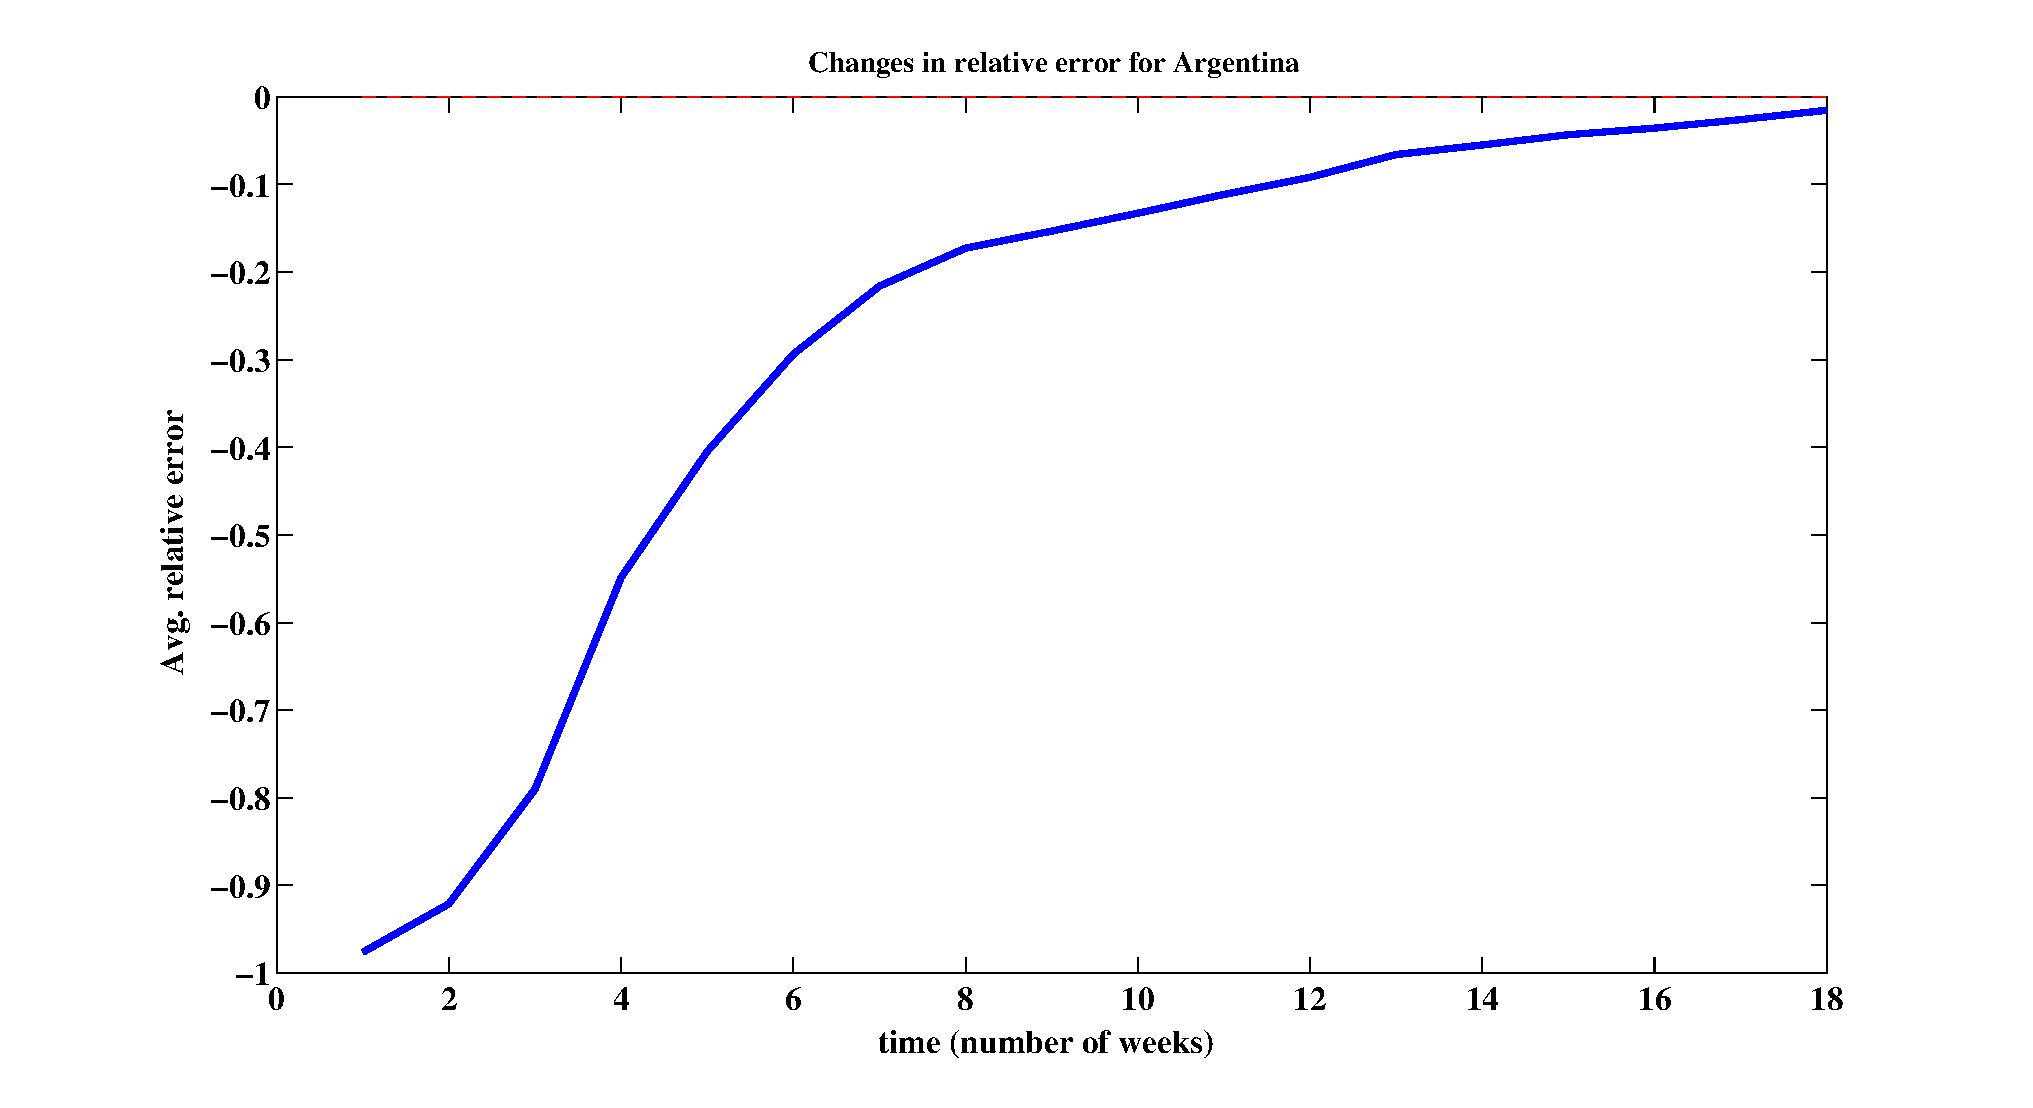
\includegraphics[width=.45\columnwidth]{fig/forpaper_AVGrelativeALLs_Argentina.eps} &
     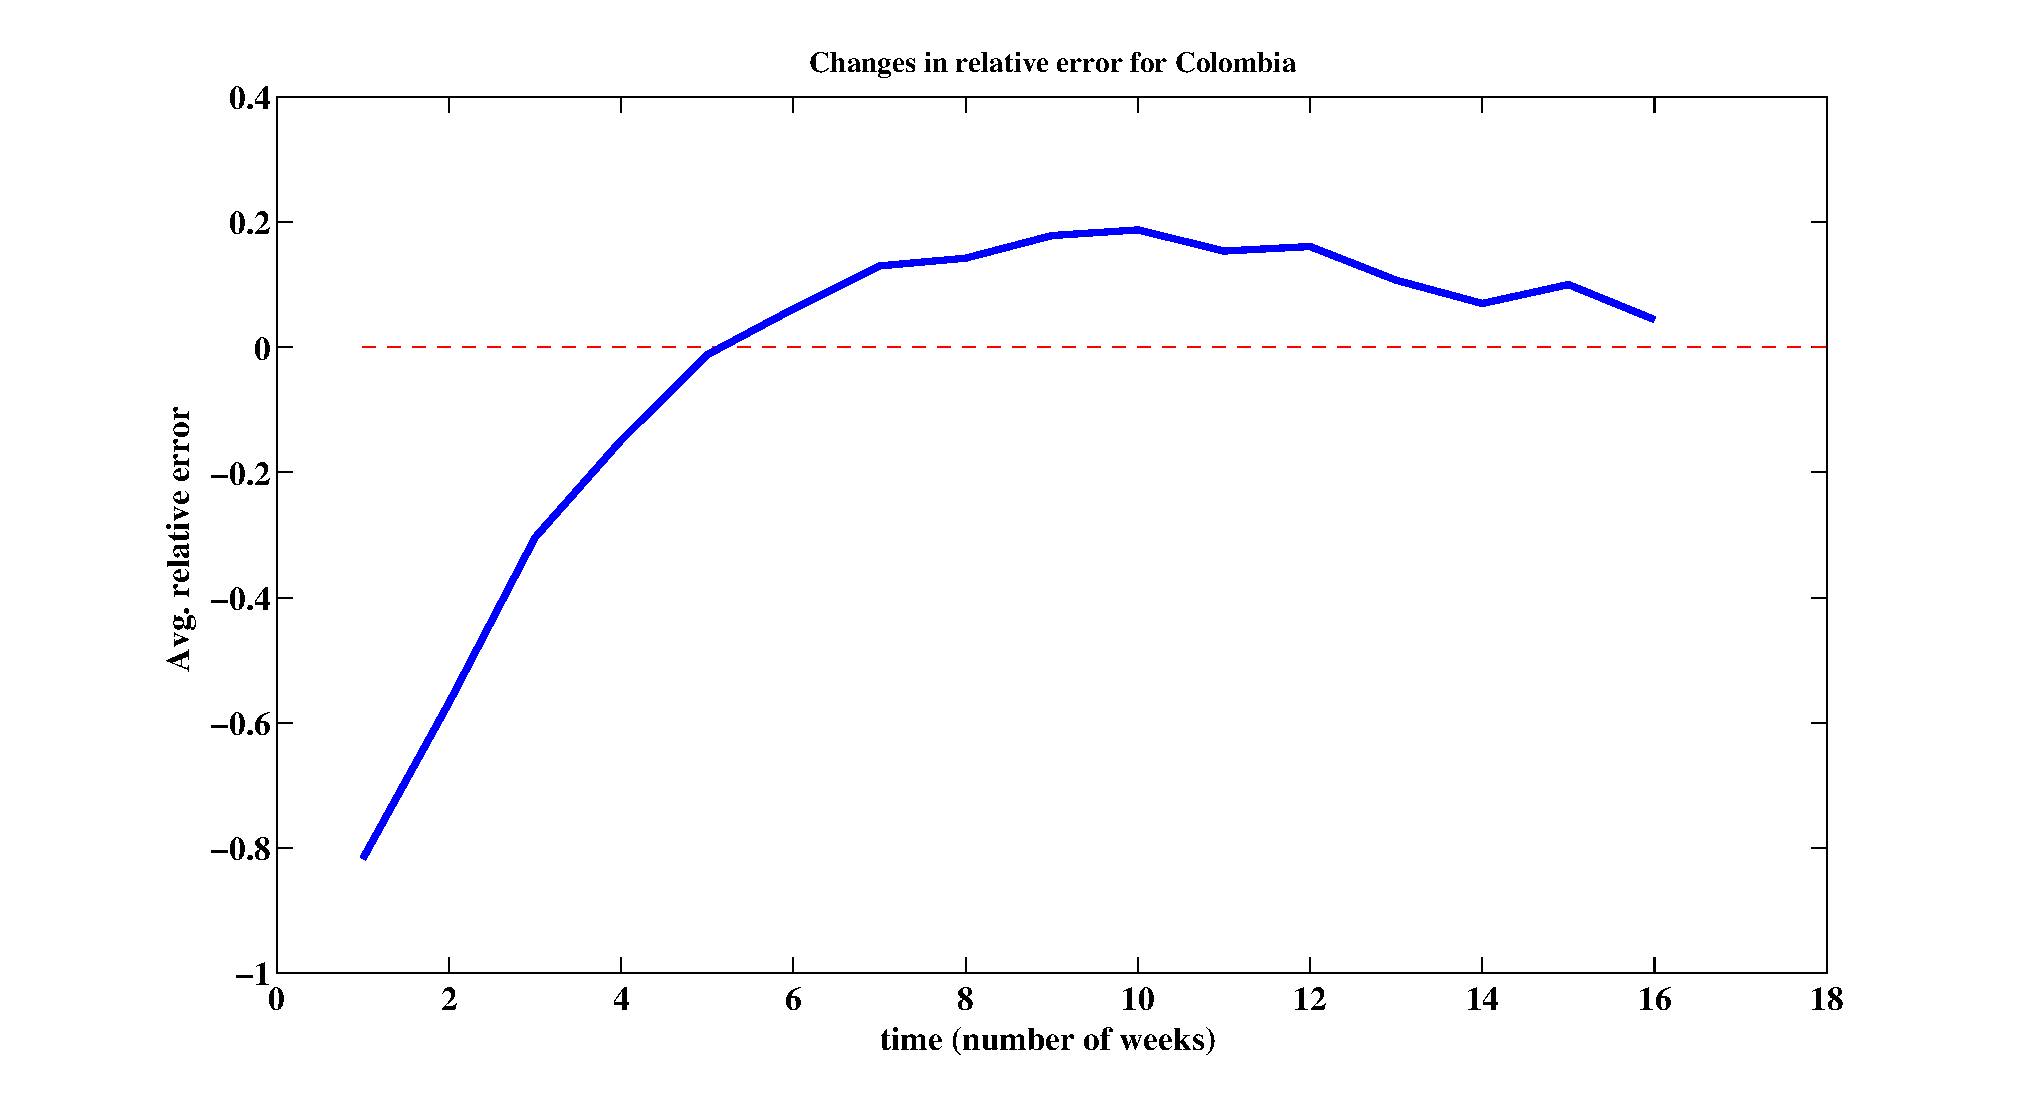
\includegraphics[width=.45\columnwidth]{fig/forpaper_AVGrelativeALLs_Colombia.eps} \\
 %    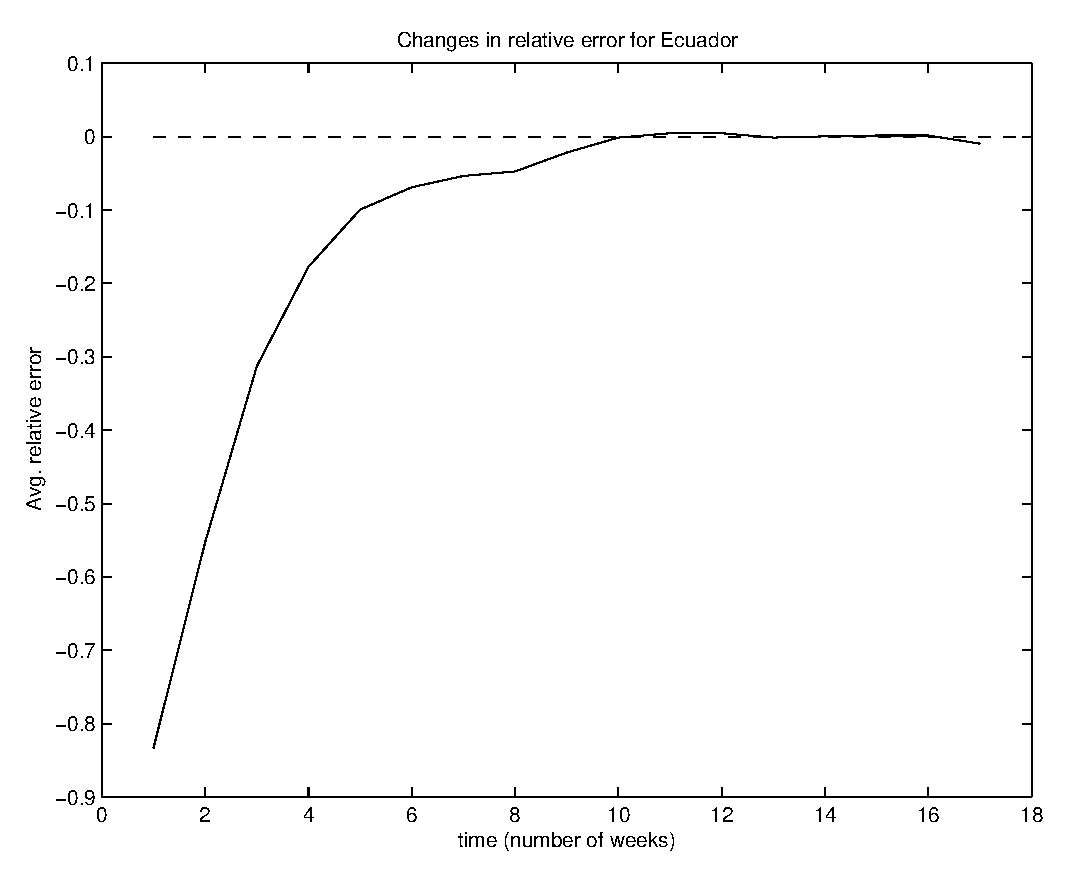
\includegraphics[width=.23\textwidth]{forpaper_AVGrelativeALLs_Ecuador.eps} &
 %    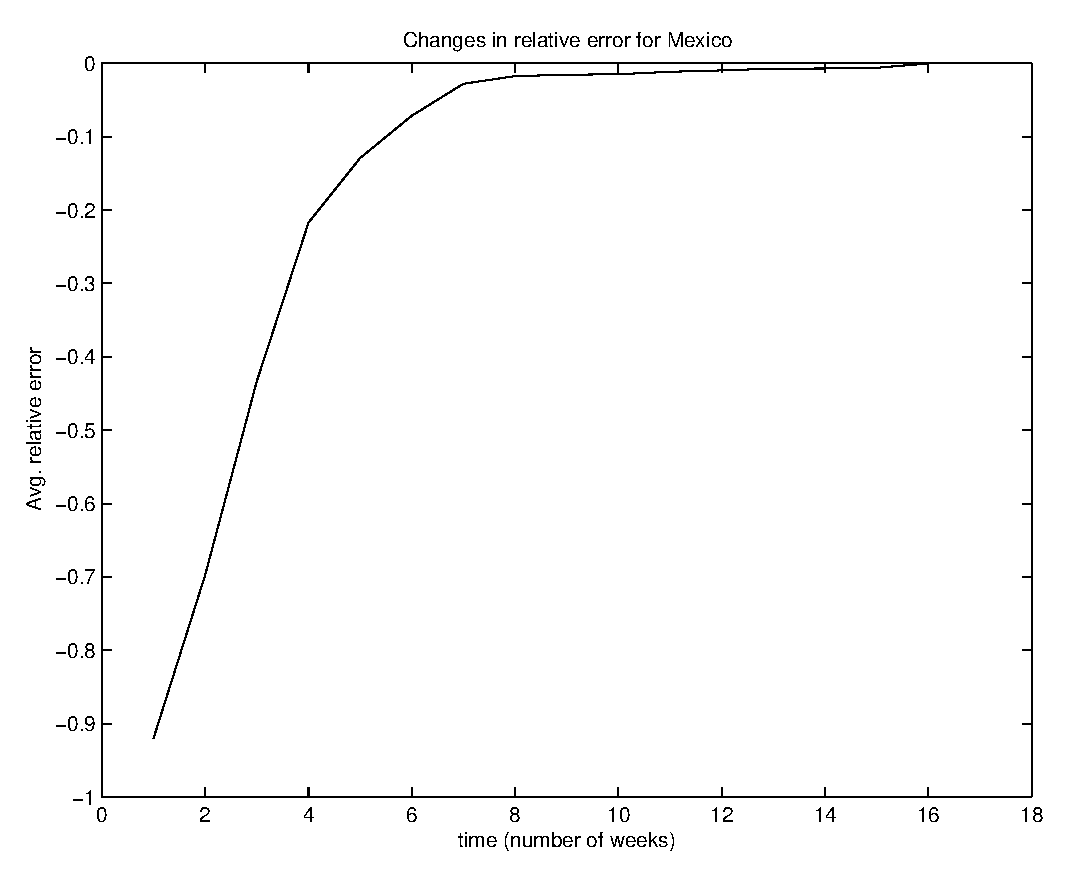
\includegraphics[width=.23\textwidth]{forpaper_AVGrelativeALLs_Mexico.eps} \\
      (a) & (b) \\ %& (c) & (d) \\
  \end{tabular}
  \caption{Average relative error of PAHO count values with respect to stable values.
  (a) Argentina
  (b) and Colombia.
%  (c) Ecuador, and
%  (d) Mexico.
  \label{fig:relerrors}
  }
\end{figure}

\begin{figure}[h]
  \centering
    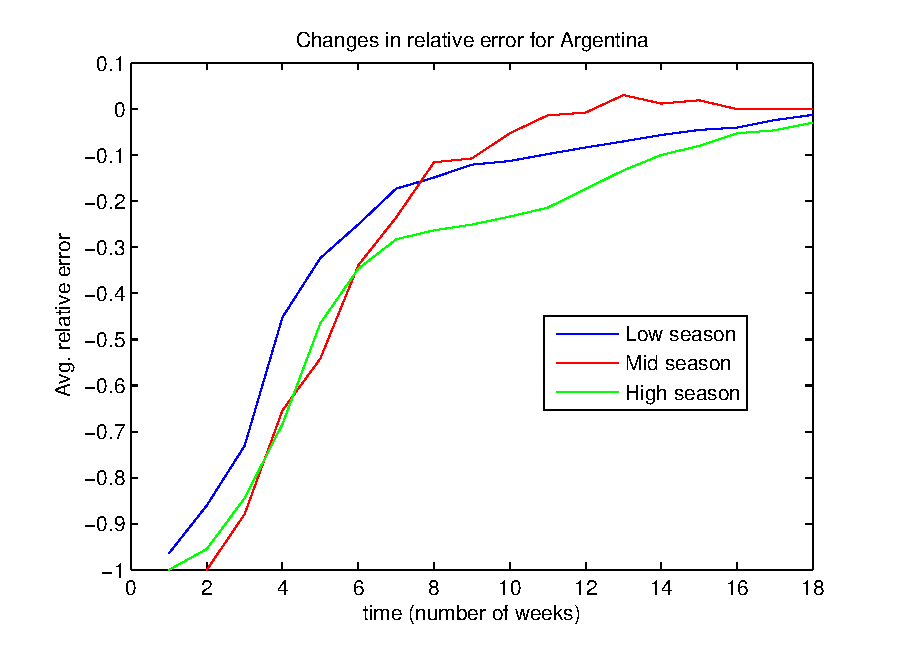
\includegraphics[width=0.5\textwidth]{fig/forpaper_seasonalAVGrelativeALLs_Argentina.eps}
  \caption{Average relative error of PAHO count values for Argentina with respect
  to their stable values for low, mid, and high seasons.}
  \label{fig:seasonal_relerrors}
\end{figure}  

% waiting for publishing stable PAHO values does not work because it is too late

At the same time, the PAHO official updates provide an indication of the number of samples
used to generate the case count estimate. Preliminary experiments show that
this size is correlated with the accuracy of ILI case counts. In other words,
in general, larger values of statistical population size results in smaller
relative errors for ILI case count. Thus using both the number of samples and the lag in 
uploading the week data, we can use machine learning techniques to revise the officially 
published PAHO estimates. Preliminary results
show that for different seasons and different countries, we encounter different
stability patterns. Therefore, any PAHO count adjustment method should be
customized for seasons and countries separately. 

Let us assume that $\dot{\mathcal{P}}$ is the set of stable PAHO counts for a
specific country. Also, assume that the sequence of updates for each stable PAHO
count value is available. In other words, for $\dot{P}_i$ we have the following
set:
 
\begin{equation}
\dot{\mathcal{P}}_i = \left \{P_i^{(1)},P_i^{(2)},...,P_i^{(m)},...  \right \}
\end{equation}
\noindent
where $P_i^{(m)}$ is the value of $P_i$ after $m$ weeks of update. 
For each stable PAHO count value, $\dot{P}_i$, there is a threshold, 
$\dot{T}_i$ such that for $m \ge \dot{T}_i$, $P_i^{(m)}$ is stable.
Hence, we have:
\begin{equation}
\dot{\mathcal{P}}_i = \left \{P_i^{(1)},P_i^{(2)},...,P_i
^{(\dot{T}_i-1)},\dot{P}_i,\dot{P}_i,...  \right \}
\end{equation}
\noindent
In other words, $P_i$ is stabilized after $\dot{T}_i$ weeks.



After recognizing high, low, and mid-season months for the country, we can
categorize each $\dot{P}_i$ to belong to one of these categories. Then, for
category S, an adjustment dataset is constructed named as $\mathcal{P}_A{^S}$
which is defined as follows:

\begin{equation}
\mathcal{P}_A{^S} = \left \{ (1,P_i^{(1)},\dot{P}_i,N_i^{(1)}),...,(m,P_i^{(m)},\dot{P}_i,N_i^{(m)}), ...  \right \}
\end{equation}

Each member of $\mathcal{P}_A{^S}$ is a tuple with four entries: the first entry denotes
the time slot that the sample belongs to; the second entry is the actual unstable
value of $P_i$; the third entry is the related stable value; and finally,
$N_i^{(m)}$ is the size of the statistical population for that week.

In the next step, a linear regression algorithm is used to adjust unstable PAHO
values. In order to adjust value of the PAHO values in the $m$th time slot of
season S, we use $\mathcal{P}_A{^S}$ set to learn $a_0$, $a_1$, $a_2$, and
$a_3$ coefficients in the following equation:

\begin{equation}
\hat{\dot{P}}_i^{(m)} = a_0 + a_1 \times m + a_2 \times P_i^{(m)} + a_3 \times N_i^{(m)}
\label{eq:correctionpaho}
\end{equation}
\noindent
where $\hat{\dot{P}}_i^{(m)}$ is the adjusted PAHO count value for the $m$th time slot.

Experimental results show that this adjustment method results in more accurate
known PAHO values. Average relative errors of the published unstable PAHO
values before and after correction for each
country are shown in Figure ~\ref{fig:avgrelerrors}. While in a few cases,
we do not experience any improvement, in countries such as Argentina and Paraguay,
we experience significant improvements.

%Some experimental results are shown in Figure ~\ref{fig:adjustedrelerrors}.

\begin{figure}[h]
  \centering
    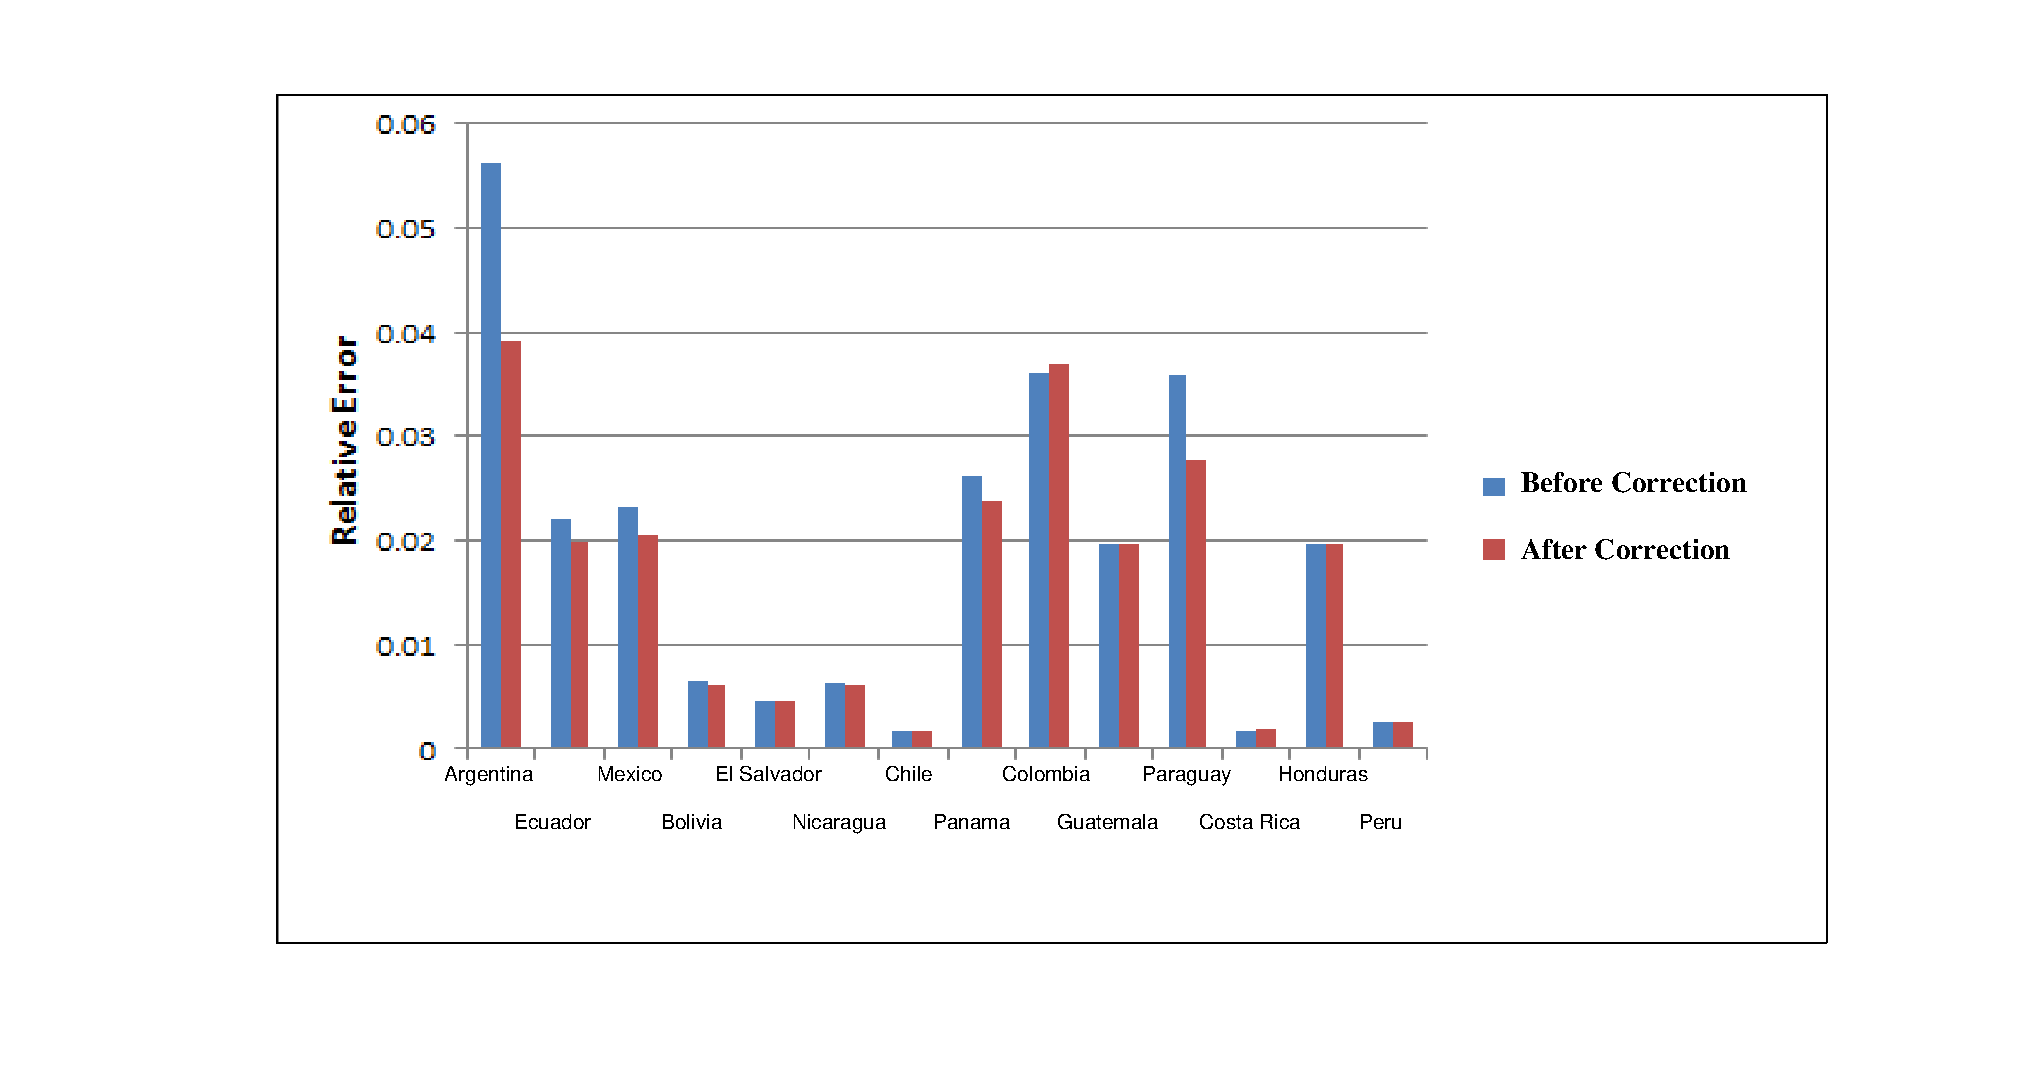
\includegraphics[width=0.5\textwidth]{fig/errs.eps}
  \caption{Average relative error of PAHO count values before and after 
  correction for different countries.}
  \label{fig:avgrelerrors}
\end{figure}

Finally, similar to Eq.~\ref{eq:correctionpaho}, in addition to $P_i^{(m)}$, one can
use only time difference ($m$) or size of population ($N_i^{(m)}$) to correct
unstable PAHO values. Effect of these corrections on overall accuracy of
predictions are explored in Section ~\ref{sec:results}.


\section{Experiments.}
% mainfile: ../ltexpprt.tex

\subsection{Reference Data.}
In this paper, we focus on 15 Latin
American countries viz. Argentina, Bolivia, Costa Rica, Colombia, Chile,
Ecuador,  El Salvador, Guatemala, French Guiana, Honduras, Mexico, Nicaragua,
Paraguay, Panama and Peru. We collected weekly ILI counts
from the official Pan American Health Organization (PAHO)
website~\cite{PAHO:2013}, {\bf every day} from January 2013 to August 2013. The
estimates downloaded every day for each country contain data from January 2010 to the latest
available week on the day of collection. 
%The downloaded data may contain some weeks with no ILI estimates and its next 
%pre-processed to fill the missing using linear interpolation. 
This dataset is stored in a database we refer to as
the {\it Temporal Data Repository} (TDR).  The TDR is also timestamped so that for
any given day, we can readily retrieve the ILI case
counts that were download on that day. This is important as historic data may be updated by
PAHO even a number of weeks after the first update.  For the purpose of experimental validation
we used the data for the period Jan 2010 to December 2012 as the static
training set. We considered Wednesdays of the weeks as a reference day within a week.  For
each Wednesday from Jan 2013 to July 2013, we used the latest available PAHO
data in TDR for that day and predicted 3 weeks from the last available week for
which the PAHO data was available. These predictions are next evaluated against
the final ILI case count as downloaded on September 1, 2013 and we report the
performance of our algorithms in Section~\ref{sec:results}. 

\subsection{Evaluation criteria.}
We evaluate the prediction accuracy of the
different algorithms using a modified version of percentage relative error:

\begin{equation} 
    \label{eq:def:accuracy} 
    \mathcal{A} = \frac{4}{N_p}\sum \limits_{t=t_s}^{t_e}\frac{|P_t -\hat{P}_t| }{max(P_t, \hat{P}_t, 10)}
\end{equation} 
where $t_s$ and $t_e$ indicate the starting and the ending
time point for which predictions were generated.  $N_p$ indicates the number of
time points over the same time period (i.e. $N_p = t_e - t_s + 1$). Note that
the measure is scaled to have values in $[0,4]$ and the denominator is
designed to not over-penalize small deviations from the true ILI case count (e.g., when
the true case count is 0 and the predicted count is 1).
It is to be noted that the accuracy metric so defined is
non-convex and is in general multi-modal. 

%The accuracy criterion was designed according the following criteria:
%\begin{itemize} 
%    \item 
%    The accuracy estimates should reflect the percentage
%    deviation in prediction rather than absolute deviation. 
%     \prithwish{should we justify this?} 
%\item The accuracy estimates must be non-negative.  \item If we
%don't consider the max operator in the denominator, even ``good'' predictions
%such as 1 for an actual count of 0 will be assigned an accuracy score of 0. As
%such we chose a threshold (here 10) for which very small deviations are not
%over-penalized. The threshold was chosen by manually inspecting the span of ILI
%case counts (which were found to lie between 0 and 2000) and subsequent
%feedback from subject experts about the ``interesting'' range of predictions.
%\end{itemize} 


\subsection{Surrogate data sources.}
For the algorithm we described in Section~\ref{sec:methods},
we used a number of different data sources as
surrogates. We considered a wide range for such surrogates comprising both
physical indicators such as weather characteristics, and also non-physical
indicators such as social network activities and user search queries.  For a
number of the non-physical indicators such as Twitter activities, the most
important part is to properly identify the keywords associated with flu so that
we can get a proper estimate of the flu-related surrogate information. This key
step is described in section~\ref{sec:keyword}, and is followed by an
explanation of the surrogates sources in section. 

\subsubsection{\label{sec:keyword} Keywords Extraction} % mainfile: ../ltexpprt.tex

The keywords relating to ILI were
organized from a seed set of words and expanded using a combination of 
time-series correlation analysis and pseudo-query expansion.
The seed set of keywords (e.g., {\em gripe}) was constructed in Spanish, 
Portugese, and English using feedback from our 
in-house subject mattter expers.

\paragraph{Pseudo-query expansion.}
Using the seed set, we crawled
the top 20 web sites (according to Google Search) associated with each
word in this set. We also crawled some expert sites such as the official CDC
website and equivalent websites of the countries under consideration, detailing the
causes, symptoms and treatment for influenza.
Additionally we crawled a few hand-picked websites such as
\url{http://www.flufacts.com} and \url{http://health.yahoo.net/channel/flu\_treatments}.
We filtered the words from these sites using standard language
processing filtering techniques such as stopword removal and Porter
stemming. The filtered set of keywords were then ranked according to 
the absolute frequency of occurrence. The top 500 words for Spanish and
English were then selected. For example, words such as {\em enfermedad}
and {\em pandemia} were obtained from this step.

\paragraph{Time-series correlation analysis.}
Next we used Google Correlate (now a part of Google Trends) to identify keywords
most correlated with
the ILI case count time-series for each country.
Once again these words were found to be a mix of 
 both English and Spanish. As an added step in this process, we also
 compared time-shifted ILI counts: left-shifted  to capture the words searched leading up to 
 the actual flu infection and right-shifted to capture the words
commonly searched during the tail of the infection. 
This entire exercise provided us some interesting terms like {\em ginger} which has been used as
a natural herbal remedy in the eastern world. We also found popular flu medications
such as {\em Acemuk} and  {\em Oseltamivir}, which are also sold under the trade name of
{\em Tamiflu} as highly correlated search queries, especially particularly for
Argentina.

\paragraph{Final filtering.}
The set of terms obtained from query expansion and correlation analysis were then 
pruned by hand to obtain a vocabulary of 151 words. We then performed a final
correlation check and retained a final set of 114 words.



We next describe the different data sources.

\subsubsection{Google Flu Trends ($\mathcal{F}$) :}
Google Flu Trends~\cite{GFT:2013} (GFT) is a tool based
on~\cite{ginsberg2008detecting} and provided by Google.org which gives weekly
and up-to-date ILI case count estimates using search query volumes. As
mentioned in~\cite{ginsberg2008detecting}, GFT is based on a regression model
from search query estimates to actual ILI case counts.  Of the countries under
consideration, GFT provides weekly estimates for 6 of them viz.  Argentina,
Bolivia, Chile, Mexico, Peru and Paraguay. As mentioned in
Table.~\ref{tb:notations}, we denote the weekly estimate of GFT data for the
country under consideration by $\mathcal{F} = \langle \mathcal{F}_1,
\mathcal{F}_2, \dots, \mathcal{F}_{T1} \rangle$. This estimate is typically at
a different scale than the ILI case counts provided by PAHO and therefore needs
to be scaled accordingly.  We collected this data weekly on Monday from Jan
2013 to Aug 2013. The data downloaded on a particular day contains the entire
time-series from 2004 to the corresponding week.  
 

\subsubsection{Google Search Trends ($\mathcal{S}$) :} Google Search Trends~\cite{GST:2013} is
another tool provided by Google. Using this tool we can download an estimate of
search query volume as a percentage over its own temporal history. This
download can be further filtered geographically over a country.  We download
the search query volumes for the 114 keywords as described in
Section~\ref{sec:keyword} every week and convert the percentage measures to
absolute values using a static dataset we downloaded on Oct 2012 when Google
Search Trends used to provide absolute query volumes. The
time series constructed using this dataset, for the country under consideration
is denoted by
$\mathcal{S} = \langle \mathcal{S}_1, \mathcal{S}_2, \dots, \mathcal{S}_{T1} \rangle$.

\subsubsection{Twitter ($\mathcal{T}$) :} 
We also collected Twitter data from Datasift~\cite{Twitter:2013},
one of the certified data resellers for
Twitter data. Using a paid data collection API, we can specify queries in
Datasift and get the corresponding filtered data.  We started with a mix of
queries targeted at collecting data from only the countries under
consideration. Using our in-house Geo coders we next processed the collected
Tweets to specific countries and then using syntactic analyzers from Basis
Enrichment~\cite{Basis:2013} we parsed the Tweet contents into ``lemma'' - root
forms of words, and also detected the Language and the part of speech for the
word under consideration.  Importantly, the Basis Enrichment step allows
differentiation between different languages (for example the Spanish word
``gripe'', meaning flu, is part of our flu keyword as opposed to the undesired
and unrelated English word ``gripe''). Also using the lemmatized versions we
can match between different parts-of-speech variations of the same word. Using
the lemma sized equivalents of our keyword dictionary we next parsed the
enriched Tweets for possible matches with flu related keywords and constructed
a time series of flu keyword weekly occurrence count. For the country under
consideration, we denote this time series by 
$\mathcal{T} = \langle \mathcal{T}_1, \mathcal{T}_2, \dots, \mathcal{T}_{T1} \rangle$.

We started collecting flu filtered Twitter Data from November 2012 and everyday
we download the corresponding Twitter time-series for each country. As shown in
Figure~\ref{fig:ili_data_pipeline}, every week we collect 10GB of raw Twitter
Data which are next enriched to 20GB of structured data. From this dataset, we
parse flu-related Tweets resulting in around 7GB of data. This data is finally
abstracted into a multivariate time series over lemmatized versions of the 114
flu related keywords and added to the TDR. 

\subsubsection{HealthMap ($\mathcal{H}$) :} 
Similar to Twitter data, we also collect flu-related
news stories using HealthMap~\cite{HM:2013}, an online global disease alert
system capturing outbreak data from over 50,000 electronic sources [including
  expert-curated accounts, such as ProMED-Mail~\cite{chase1996promed}, news media
and official reports from local, national and global public health
organizations.] Using this service we receive flu-related news as a daily feed
which is similarly processed using Basis Enrichment and further filtered to get
a multivariate time series over  lemmatized version of the keywords. For a
particular country, we denote this time series by: 
$\mathcal{H} = \langle \mathcal{H}_1, \mathcal{H}_2, \dots, \mathcal{H}_{T1} \rangle$.

While Twitter Data is more suitable to look for general public response, the
HealthMap data provides more detailed information but may capture the trends
more slowly than the Twitter Data. Thus each of these sources offers utility in
capturing different surrogate signals: Twitter Data offers leading but noisy
indicators whereas HealthMap Data provides a slightly delayed but more reliable
indicator.

\subsubsection{OpenTable ($\mathcal{O}$) :}
We also use data on trends of restaurant table reservations, as initially 
found in~\cite{elaine2013opentable} to be a potential early indicator for
outbreak surveillance, as another surrogate for ILI detection.
This novel data stream is based on the
postulate that higher than average number of restaurants with table
availabilities in a region can serve as an indicator of an event of interest
such as increase in flu cases. Table availability was monitored using OpenTable
~\cite{Opentable:2013}; an online restaurant reservation site with 28,000 restaurants at the time
of this writing. Daily searches were performed starting from September 2012 for
a table for two persons at lunch and dinner; between 12:30-3pm, and between
6-10:30pm. Data was collected for Mexico by city (Cancun, Mexico City, Puebla,
Monterrey, and Guadalajara) and for the entire country. The daily proportion
(proportion used due to changes in the number of restaurants in the system) of
restaurants with available tables was aggregated as a weekly time-series and
is denoted by 
$\mathcal{O} = \langle \mathcal{O}_1, \mathcal{O}_2, \dots, \mathcal{O}_{T1} \rangle$.


%--Since we monitored ten regions at twenty search times, this resulted in 200
%distinct time-series curves.
\begin{figure} 
  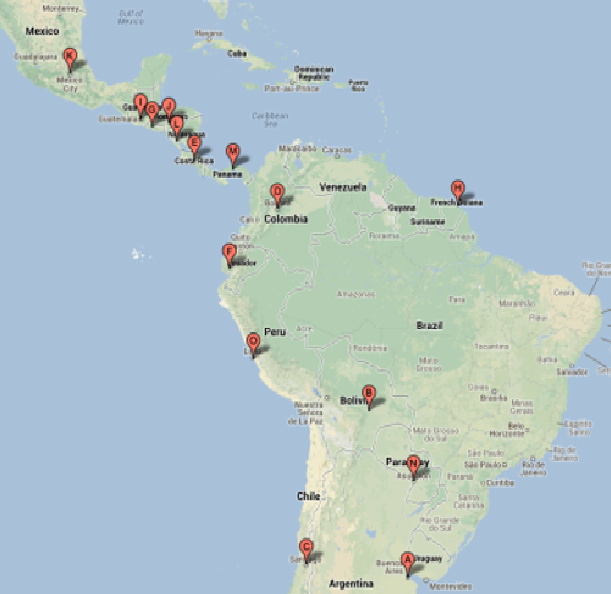
\includegraphics[width=3.33in]{fig/humidity_centers.pdf}
  \caption{\label{fig:surveillance} PAHO surveillance centers for the 15 Latin
  American countries.}
\end{figure}

\subsubsection{Weather Data ($\mathcal{W}$) :}
All of the previously described data sources can
be termed as `non-physical' indicators. These data sources can work as indirect
indicators about the state of the population with respect to flu by exposing
different population characteristics. At the same time, meteorological data can
be considered a more direct and `physical' driver of influenza transmission
~\cite{flu_humidity_physical}. It has been shown
in~\cite{Shaman_orig_humidity_link, Shaman_humidity_USA, ref9}
that absolute humidity can be directly used to predict the onset of influenza
epidemics. Here, we collected several other meteorological factors such as
temperature and rainfall in addition to humidity from the Global Data
Assimilation System (GDAS) which is a series of weather models run by National
Weather Service's National Centers for Environmental Prediction that provides
detailed meteorological data in near real-time across the globe.  We accessed
the data via an archive hosted by NASA (\url{http://ladsweb.nascom.nasa.gov/})
~\cite{HD:2013}, and provided in GRIB format. By specifying the resolution and
the geographical boundaries we can collect the data for the countries under
consideration to a resolution of 1 degrees lat/long interval. However, looking
at all the lat/long for a country can often lead to noisy data. As such we
filtered the downloaded data and parsed the meteorological data only around the
PAHO surveillance centers as shown in Figure~\ref{fig:surveillance}. We also
aggregate this data using weekly averages and for a particular country we
represent the time resultant time series by: 
$\mathcal{W} = \langle \mathcal{W}_1, \mathcal{W}_2, \dots, \mathcal{W}_{T1} \rangle$.

We collected this data weekly from Jan 2013 to August 2013. 


\subsubsection{Temporal Data Repository}
All of the described data sources were
added to a temporal database, ``Temporal Data Repository'' (TDR). Some of the
data sources such as the Weather Data, Twitter Data, HealthMap Data and
OpenTable data once downloaded doesn't change. Also at the time of download
these datasets are updated till the corresponding day.  Thus to extract the
data available at a certain time point for these data sets we can simply
consider the corresponding truncated time series from the latest data. However,
Statistics like Google Search Trends and the PAHO ILI case counts exhibit
variability in past data. In these cases, the actual time series for these datasets are
stored in TDR with the corresponding timestamps. Thus given any time point,
using TDR we can quickly reference the data available at that point of time and
run our algorithm to simulate a prospective analysis scenario.  The entire data
collection process is depicted pictorially in
Figure~\ref{fig:ili_data_pipeline}.





\section{Discussions.}
% mainfile: ../ltexpprt.tex
\begin{table*}[tb!]
\scriptsize
\centering
\captionsetup{font=scriptsize}
\caption{\label{tb:comparison_single}  Comparing forecastng accuracy of models using individual sources.}
\vspace{-1em}
\begin{tabular}{|*{18}{c|}}
\hline
Model               & Sources       & AR & BO & CL & CR & CO & EC & GF & GT & HN & MX & NI & PA & PY & PE & SV & All\\
\hline \hline
\multirow{5}{*}{MF} & $\mathcal{W}$ &2.78&2.46&2.39&2.14&2.70&2.22&2.12&2.63&2.52&2.73&2.31&2.21&2.49&2.77&2.61&2.47\\ 
                    & $\mathcal{H}$ &2.81&2.31&2.22&1.92&2.43&2.04&2.11&2.57&2.33&2.48&2.39&2.15&2.18&2.47&2.33&2.32\\ 
                    & $\mathcal{T}$ &2.37&2.35&2.18&2.03&2.21&2.12&1.83&2.12&2.29&2.03&1.89&2.06&1.96&2.20&2.21&2.12\\ 
                    & $\mathcal{F}$ &2.34&2.11&2.29& N/A& N/A& N/A& N/A& N/A& N/A&2.71& N/A& N/A&2.31&2.24& N/A&2.33\\ 
                    & $\mathcal{S}$ &2.48&2.21&2.33&2.04&2.31&2.21&1.93&2.03&2.15&2.51&2.42&2.52&2.33&1.93&2.30&2.24 \\ 
\hline
\multirow{5}{*}{NN} & $\mathcal{W}$ &2.92&2.93&2.63&2.52&2.66&2.51&2.71&2.82&2.59&2.62&2.55&2.59&2.61&2.80&2.52&2.66\\ 
                    & $\mathcal{H}$ &2.73&3.10&2.42&2.27&2.83&2.64&2.43&2.25&2.71&2.31&2.61&2.35&2.43&2.39&2.52&2.53\\ 
                    & $\mathcal{T}$ &2.72&2.86&2.31&2.62&2.77&2.52&2.71&2.66&2.51&2.44&2.13&2.01&1.77&2.51&2.20&2.45\\ 
                    & $\mathcal{F}$ &2.11&2.21&2.33& N/A& N/A& N/A& N/A& N/A& N/A&2.19& N/A& N/A&2.41&2.32& N/A&2.26\\ 
                    & $\mathcal{S}$ &2.51&2.31&2.41&1.81&2.52&2.41&2.12&2.29&2.51&2.13&2.61&2.14&2.51&1.87&2.12&2.28 \\ 
\hline
\multirow{5}{*}{MFN}& $\mathcal{W}$ &2.99&3.01&2.88&2.53&2.78&2.81&2.77&2.83&2.61&2.70&2.56&2.66&2.82&2.79&2.51&2.75\\ 
                    & $\mathcal{H}$ &2.81&3.13&2.63&2.58&2.91&2.77&2.57&2.63&2.73&2.50&2.61&2.54&2.51&2.69&2.61&2.68\\ 
                    & $\mathcal{T}$ &2.74&3.03&2.51&2.64&2.83&2.51&2.81&2.71&2.60&2.48&2.13&2.55&2.19&2.57&2.31&2.57\\ 
                    & $\mathcal{F}$ &2.33&2.41&2.34& N/A& N/A& N/A& N/A& N/A& N/A&2.69& N/A& N/A&2.54&2.48& N/A&2.46\\ 
                    & $\mathcal{S}$ &2.61&2.44&2.55&2.22&2.61&2.52&2.71&2.31&2.62&2.48&2.61&2.31&2.53&2.23&2.13&2.46\\ 
\hline
\end{tabular}
\vspace{-1em}
\end{table*}

\begin{table*}[tb!]
  \scriptsize
  \centering
\captionsetup{font=scriptsize}
  \caption{\label{tb:comparison_ensemble}Comparison of prediction accuracy while combining all data sources
  and using MFN regression.}
\vspace{-1em}
  \begin{tabular}{|p{1.5cm}|*{16}{l|}}
\hline
Fusion Level& AR & BO & CL & CR & CO & EC & GF & GT & HN & MX & NI & PA & PY & PE & SV & All\\
\hline \hline
Model       &3.12&3.22&3.03&2.88&2.98&3.13&2.87&2.99&2.87&3.00&2.77&2.82&2.81&2.92&2.87&2.95\\ 
Data        &3.01&2.97&3.13&2.87&2.86&3.04&2.91&2.88&2.72&2.89&2.70&2.60&2.88&2.81&2.92&2.88\\ 
\hline
\end{tabular}
\vspace{-1em}
\end{table*}
\begin{table*}[tb!]
  \scriptsize
  \centering
\captionsetup{font=scriptsize}
  \caption{\label{tb:moving} Comparison of prediction accuracy while using model level fusion 
  on MFN regressors and employing PAHO stabilization.}
\vspace{-1em}
\begin{tabular}{|p{1.5cm}|*{16}{c|}}
\hline
Correction Method& AR & BO & CL & CR & CO & EC & GF & GT & HN & MX & NI & PA & PY & PE & SV & All\\
\hline \hline
None             &3.12&3.22&3.03&2.88&2.98&3.13&2.87&2.99&2.87&3.00&2.77&2.82&2.81&2.92&2.87&2.95\\ \hline
Weeks Ahead      &3.15&3.24&3.04&2.87&2.97&3.17&2.87&2.99&2.88&3.05&2.77&2.91&3.02&2.91&2.88&2.98\\ \hline 
Num samples      &3.20&3.24&3.03&2.88&2.96&3.12&2.87&3.01&2.89&3.12&2.78&2.92&3.04&2.91&2.87&2.99\\ \hline
Combined         &3.21&3.24&3.05&2.89&2.96&3.19&2.87&3.00&2.89&3.13&2.77&2.93&3.08&2.92&2.88&3.00\\ 
\hline
\end{tabular}
\vspace{-1em}
\end{table*}

\begin{table*}[tb!]
  \scriptsize
  \centering
\captionsetup{font=scriptsize}
  \caption{\label{tb:Ablation} Discovering importance of sources in Model level fusion on MFN 
  regressors by ablating one source at a time.}
\vspace{-1em}
\begin{tabular}{|*{17}{c|}}
\hline
Sources & AR & BO & CL & CR & CO & EC & GF & GT & HN & MX & NI & PA & PY & PE & SV & All\\
\hline 
\hline
All               & 3.21& 3.24& 3.05& 2.89& 2.96& 3.19& 2.87& 3.00& 2.89& 3.13& 2.77& 2.93& 3.08& 2.92& 2.88& 3.00\\
w/o $\mathcal{W}$ & 2.91& 2.99& 2.77& 2.71& 2.61& 2.59& 2.66& 2.69& 2.49& 2.78& 2.62& 2.87& 2.60& 2.43& 2.67& 2.69  \\
w/o $\mathcal{H}$ & 3.04& 2.85& 2.89& 2.56& 2.81& 2.77& 2.61& 2.75& 2.75& 2.82& 2.57& 2.75& 2.51& 2.87& 2.71& 2.75  \\
w/o $\mathcal{T}$ & 2.92& 3.14& 2.95& 2.61& 2.72& 2.81& 2.88& 2.79& 2.61& 2.93& 2.74& 2.63& 2.79& 2.74& 2.81& 2.80  \\
w/o $\mathcal{S}$ & 3.19& 3.11& 2.92& 2.64& 2.69& 2.70& 2.89& 2.88& 2.78& 3.07& 2.75& 2.91& 2.80& 2.71& 2.86& 2.86  \\
w/o $\mathcal{F}$ & 3.20& 3.12& 2.88& 2.89& 2.96& 3.19& 2.87& 3.00& 2.83& 3.02& 2.77& 2.93& 2.98& 2.88& 2.88& 2.96  \\
\hline
\end{tabular}
\vspace{-1em}
\end{table*}
\begin{table}[t]
  \scriptsize
\centering
\captionsetup{font=scriptsize}
\caption{\label{tb:opentable}  ILI case count prediction accruacy for Mexico using OpenTable data as a single source, and
by combining it with all other sources using model level fusion on uncorrected ILI case count data.}
\vspace{-1em}
\begin{tabular}{|p{1.5cm}|*{2}{l|}p{2cm}|}
\hline
Method& Lunch & Dinner & Lunch \& Dinner \\
\hline \hline
MF   & 1.92 & 2.23 & 2.31 \\
NN   & 1.99 & 1.83 & 2.11 \\
MFN  & 2.11 & 2.31 & 2.44 \\
Model Fusion & 2.96 & 2.87 & 2.99 \\
\hline
\end{tabular}
\vspace{-3em}
\end{table}

We present an exhaustive set of experiments evaluating our algorithms 
over 6 months of predictions 
from Jan 2013 to August 2013. The final estimates of ILI case counts are stable according
to the estimates downloaded from PAHO on Oct 1, 2013. All models considered here were
used to forecast 2 weeks beyond the latest available PAHO ILI estimates. 
Key findings
are presented in 
Table.~\ref{tb:comparison_single}. We analyze 
some important observations from this table next.




{\noindent \textbf{Can we `beat' Google Flu Trends with our custom dictionary?}}  
The key difference between Google Flu Trends and Google Search Trends is that the former uses a closed dictionary whereas
we constructed the dictionary to use with GST.
As can be seen Table~\ref{tb:comparison_single},
for majority of the common countries (countries for which data from both GST and GFT
is present), regressors running on GST consistently 
outperform those running on GFT (with Mexico and Peru being the exception).
Thus we posit that the GST model devised here is a sufficiently close approximation to GFT, 
with the added advantages of having access to raw level data and being available for more countries 
than GFT (among the 15 countries we consider, only 6 of them are present in the GFT database).

{\noindent \textbf{Which is the optimal regression model?}} From Table~\ref{tb:comparison_single}, we can also
analyze the three different regressors proposed in Section~\ref{sec:methods} with respect to overall accuracy.
With respect to each individual source, we can see that matrix factorization with nearest 
neighbor embdedding (MFN) performs the best in average over the countries.
For some countries such as Panama, when using only Google Search Trends, MFN
performs poorer than vanilla MF; nevertheless the average accuracy over all countries for any given
data source is best when using MFN.



{\noindent \textbf{Which is the best strategy to combine
multiple data sources?}} 
As shown in Table~\ref{tb:comparison_ensemble}, in overall,
model level fusion works better than data level fusion.
For 8 of the 15 countries, model level fusion works
appreciably better than data level fusion, while the reverse trend is seen for 4 other countries. 
This showcases the importance of considering both kinds of fusion depending on the country of interest.


{\noindent \textbf{How effective are we at forecasting a moving PAHO target?}} 
As shown in Table~\ref{tb:moving}, 
our
corrected estimates 
using both the number of samples and 
the {\it weeks ahead} from the upload date are generally better. It is instructive to note that
our correction strategy is
able to increase the overall accuracy only by a score of approximately 0.05 over all the countries, 
for some countries such as Mexico and Argentina (for which the data update is typically noisy) we obtain 
a substantial imporovement of scores. This suggests that the correction strategy may be selectively applied 
when forecasting for certain countries. 




{\noindent \textbf{How do physical vs social indicators fare against each other?}} 
From Table~\ref{tb:comparison_single}, we 
see that the data source with the best single accuracy happens to be the physical indicator source, i.e.,
weather data. However, Table~\ref{tb:Ablation} conveys a mixed story. Here we conduct an {\it ablation test},
wherein we remove one data source at a time from our model level MFN fusion framework and contrast accuracies.
While removing the weather data degrades the accuracy score the most, removing the social indicators also degrades
the score to varying degrees.
Thus we posit that it is important to consider both the physical 
and social indicators to get a refined signal about the prevalent ILI incidence in the population.

%\begin{itemize}
  %%\item Table~\ref{tb:comparison_single} Comapring the three regression methods (one for each source and country). 
  %%\item Discussion GST vs GFT.
  %%\item Table~\ref{tb:comparison_ensemble} Which Ensembling method to use.
  %%\item Table~\ref{tb:Ablation} Ablation tests
  %%\item Table~\ref{tb:moving} Forecasting moving target (three different methods).
  %\item Opentable data (more analysis... make this with only Mexico.. just a single plot may suffice). 
%\end{itemize}


{\noindent \textbf{How relevant is restaurant reservation data to forecasting ILI?}} 
All the results thus far do not consider the OpenTable reservation data, since this source is available only for
Mexico (among the countries studied here). We considered table availability for different time ranges and compared
performance using our MFN model. As Table~\ref{tb:opentable} demonstrates, we obtain the best performance when
considering both lunch and dinner reservation data. Nevertheless, we have observed that including this source
as part of the ensemble decreases the overall accuracy by 0.01 over the uncorrected ILI case count data.
Thus it is our opinion that although the reservation data could exhibit some signals about prevalent ILI
conditions, it likely is also a surrogate for non-health conditions (e.g., social unrest) which must be factored
out to make the data source more useful.

Finally we present Figure~\ref{fig:accuracies} where we compare
the overall prediction accuracies for different countries. We show the best
accuracy achievable from an individual source, before showing how we improve this 
performance by using both data level and model level fusion of the different sources and finally 
present the accuracies when model level fusion of MF regressors is applied on the corrected PAHO 
estimates rather than the raw ones. As can be seen, we progresively increase our accuracies
with the corrected PAHO estimates providing the final increase in predictive power to 
our model level fusion framework.



\section{Conclusions and Further Work.}
% mainfile: ../ltexpprt.tex
To forecast ILI over a range of Latin American countries,
we have explored a gamut of options pertaining to data sources, fusion possibilities, and corrections to
track a moving target. Our results demonstrate that there are significant opportunities to
improve forecasting performance and selective superiorities among data sources that can be leveraged.
Our future work focuses on reconciling the phenomenological models developed here with true epidemiological
models to that we can develop not just near-term forecasts as done here but also identify long-range 
characteristics of the epidemic as it unfolds.


%FOR NOW. TO be replaced by the bbl
\bibliographystyle{IEEEtran}
\bibliography{references}

%\begin{thebibliography}{99}

%\bibitem{GUIDE}
%R.~E. Bank, {\em PLTMG  users' guide, edition 5.0}, tech. report,
  %Department of Mathematics, University of California, San Diego, CA, 1988.


%\bibitem{LIU}
%J.~W.~H. Liu, {\em A compact row storage scheme for cholesky factors
  %using elimination trees}, ACM TOMS, 12 (1986), pp.~127--148.

%\bibitem{LIU2}
%\sameauthor , {\em The role of
  %elimination trees in sparse factorization}, Tech. Report CS-87-12,Department
  %of Computer Science, York University, Ontario, Canada, 1987.

%\bibitem{ROSE72}
%D.~J. Rose, {\em A graph theoretic study of the numeric solution of
  %sparse positive definite systems}, in Graph Theory and Computing, Academic  Press, New
%York, 1972.


%\end{thebibliography}
\end{document}
